% background
% brief review of previous research (cite)
% reson why the research was undertaken
% Hypothesis
% explenation of techniques and why they ve been chosen
% objectives = what you hope to achieve
% brief reference to the main outcome
\section{Introduction}
\label{sec:Introduction}

Luminescence is a phenomenon where a sample of any kind get energetically excited and thus emits light of a material and structural specific spectrum.
But also, it is used in nowadays consumer technologies like TV screens. 
In this case, photoluminescence is used to characterize the specifications of three samples, which are semiconductor compounds of the same elements but in different concentrations.
In the following, the samples, as well as the process of photoluminescense, are recalled.

\subsection{Photoluminescense in Semiconductors}
\label{sec:PLS}

Semiconductors are characterized by a bandgap of $\SI{2}{\eV}$ to $\SI{4}{\eV}$, an almost completely filled valence band and an almost completally empty conductance band \cite[391]{festkorperphysik}.
Here, a lightsourse like a LED or Laser is able to excite some electrons from the valence band up into the conductance band, as long as the photoenergy is bigger then the bandgap of the sample.
The electrons loose energy by exciting lattice vibrations, and by reaching the minimum of the conductance band, they may recombine with a hole in the valence band, emmitting a photon with the energy of the band gap.
Here, the equation
\begin{equation}
    h\nu = E_{\text{g}}
\end{equation}\label{eq:h}
holds, where $\nu$ is the photons frequency, and $E_\text{g}$ the band gap.
One easily can see, that the expected frequency of the emitted photons is smaller than the frequency of the pump. 
Nevertheless, due to thermal affects a thermal spread along the energy of the bandgap, and thus a widening of the spectrum around a $\lambda_\text{peak}$ is expected.
Using a spectrometer, this wavelengh can be found, and used to estimate the bandgap energy
\begin{equation}
    E_{\text{g}} = \frac{h\c}{\lambda_\text{peak}}.
\end{equation}

\subsection{Samples}
\label{sec:samples}

There are three $\ce{CdS_x Se_{1-x}/ZnS}$ samples to analyze, where all of them can be described as quantum dots, as the $\ce{ZnS}$ has a bigger bandgap than the $\ce{CdS_xSe_{1-x}}$ molecule, 
thus it acts as a potential barrier.
This provides a confinement potential. The impact of quantum dots on the spectrum is referred in chapter \ref{sec:QD}.
The molecules of $\ce{CdS_x Se_{1-x}/ZnS}$ with a unknown concentration $x$ are submerged in tulene.
The relation between the concentration $x$ and the material's bandgap is mentioned in chapter \ref{sec:SemAll}.

Another sample is methylammonium lead bromide ($\ce{MAPbBr_3}$), a hybrid perovskite single crystal, which is a material used in new approaches of optoelectronic devices.

\subsection{Semiconductor alloys}
\label{sec:SemAll}

Under preserving the lattice structure of the crystal but subseducing one compuond of a semiconductor alloy, the bandgap and the lattice constant changes.
The dependency can be non-lineary, thus a bowing parameter $b$ is introduced. 
The dependency of the bandgap from the subsedution of $\ce{S}$ with $\ce{Se}$ in an alloy with $\ce{Cd}$, quantified by the mentioned concentration (of $\ce{S}$) is given by
\begin{align*}
    E_g(\ce{Cd S_x Se_{1-x}}) &= x \times E_g(\ce{Cd S}) + (1-x) \\ &\times E_g(\ce{Cd Se}) - bx(1-x).
\end{align*}\label{eq:E-G}

\subsection{Quantum dot spectra}
\label{sec:QD}

A quantum dot is a one-dimensional potential well, in which the solution of the Schrödinger equation for the electrons gives a discrete energy spectrum, comparable to the one of a single atom.
The lowest available energy state depends on the size of the smallest dimension which here is given by the molecule size.
In the undertaken photoluminescence measurement the emission primarily comes from a relaxation of the lowest energy electron in the conductance band to the highest energy state of the valence band, as explained in chapter \ref{sec:PLS}.
Thus, the dimension of the quantum dot, determining the lowest energy state, is the parameter to set, in order to get the samples $\ce{S}$ concentation out of the spectral information.

\begin{figure*}
  \centering
  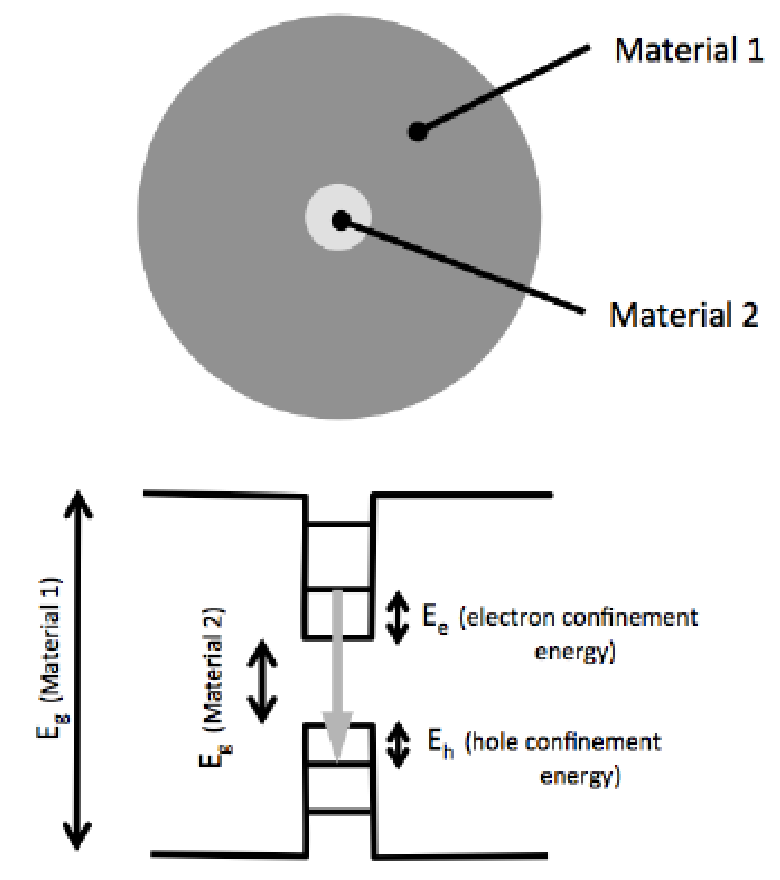
\includegraphics[width=0.35\textwidth]{graphics/QD.png}
  \caption[width=0.4\textwidth]{Structure of a spherical quantum dot and the potential well, created by the surrounding of a material with a bigger bandgap. The optical excitation energy depends not only on the samples band gap $E_g$, but also on the confinement energies due to the quantum dot dimensions\cite{instruction}.}
  \label{fig:QD}
\end{figure*}

As seen in figure \ref{fig:QD}, the optical transition energy is given by
\begin{equation}
    h \nu = E_g + E_e + E_h,
\end{equation}
where $E_g$ is the fundamental bandgap of the material and $E_{e/h}$, the confinement energy for electrons/holes.
Assuming a symetrical quantum dot with a radius $r$, and a linearly on the composition dependent effective mass of the electrons and holes
\begin{align*}
m_e^*(\ce{Cd S_x Se_{1-x}}) &= x m_e^*(\ce{Cd S}) \\ &+ (1-x)m_e^* (\ce{CdSe}) \\
m_h^*(\ce{Cd S_x Se_{1-x}}) &= x m_h^*(\ce{Cd S}) \\ &+ (1-x)m_h^* (\ce{CdSe}),
\end{align*}
for the first confined state one gets
\begin{equation}
    h \nu = E_g + \frac{h^^2}{8er^^2}(\frac{1}{m_e^*} + \frac{1}{m_h^*}).
\end{equation}\label{eq:QD}

\subsection{Experimental setup}
\label{sec:setup}

As lightscources there are used a UV 395 LED as well as a 375nm LDH laser Diode.
The Thorlabs CCS200 Spectrometer is connected with a fiber optic which can be positioned next to the sample. 
In order to minimalize the noise of the exciting light source, a perpendicular positioning to it is used.
The Spectrometer uses a grating in order to project one wavelength onto a CCD linear image sensor.
The wavelength intensity scan can be acquired by moving a mirror. This happens automatically, such that a wavelength-intensity plot is available in the acquisition software.

As there is expected to have noise from external light sources during the experiment, a background measurement for the LED setup is needed.
This can be substracted from the signal later on.
For the laser setup, a darkening curtain is used. 
To overcome statistical fluctuations, the integration time of the acquisition is set to the highest possible level without saturation occurring.
